\documentclass[10pt]{article}
\usepackage[margin=1in]{geometry}
\usepackage{amsmath,amssymb,amsthm}
\usepackage{booktabs}
\usepackage{graphicx}
\usepackage{xcolor}
\usepackage[hidelinks]{hyperref}
\usepackage{enumitem}
\setlist{itemsep=2pt,topsep=4pt}
\newtheorem{theorem}{Theorem}
\newtheorem{lemma}{Lemma}
\newtheorem{proposition}{Proposition}
\newtheorem{assumption}{Assumption}
\theoremstyle{remark}
\newtheorem{remark}{Remark}
\newcommand{\pending}[1]{\textcolor{red}{[#1]}}

\title{Exact Conformance Tests for Speculative Decoding\\ and Samplers in LLM Inference Engines}
\author{Auden Venn\\ Independent Researcher}
\date{November 2026}

\begin{document}
\maketitle

\begin{abstract}
Local LLM inference engines now enable speculative decoding and multi-token prediction (MTP) by default. They document exactness properties such as ``correct at any temperature'' or ``bit-for-bit what decoding one token at a time produces.'' We give two tests of such properties and state the conditions under which each is exact.
\begin{itemize}
\item \emph{L1} applies the randomized probability integral transform (PIT) to each emitted token under the distribution the engine declares. It is exact under adaptive generation whenever the declared distribution is fixed before the token is drawn. It stays exact under three operations: selection by rules fixed before the draw, coarsening to tie classes or a reported top-$K$, and screening of positions whose declared distribution cannot be computed exactly.
\item \emph{L3} is an exact permutation test between two arms scored by any fixed reference model.
\end{itemize}

On synthetic ground truth with realistic sequence lengths, L1 detects nine sampling-rule bug classes at deployment settings. Five are detected within 3k tokens, mostly through impossible tokens. Two errors in the rejection path, resampling from the target and an untransformed residual, need about 100k. $\chi^2$ counting of the first token after fixed prefixes sees those two far sooner, but it is blind to bonus-token and state errors. L3 is calibrated and detects state errors, but it has little power against subtle acceptance errors at audit sizes.

We also study the history of an unmerged MTP pull request to mlx-lm. Every buggy commit we tested fails at least one test, and every correct one passes. One commit contains a recurrent-state contamination, flagged and removed by its author within 24 minutes. It moves per-token distributions 28--53$\times$ the numerical floor; L1 cannot see it, and L3 can. Correct greedy speculation diverges from plain decoding at 0.6\% per token, at logit near-ties.

An audit of four engines on Apple silicon finds no evidence of a speculation effect and no speculative-decoding error. Reading source code, followed by targeted tests, found two silent sampler deviations:
\begin{itemize}
\item raceline, developed by the author, kept only the top 1024 tokens when top-$k{=}0$; this is fixed in 0.8.1;
\item kapitsa clamps top-$k$ to 32; this has been reported upstream.
\end{itemize}
We release \texttt{lossless}, an engine-agnostic tool, at \url{https://github.com/audenvenn/lossless}.
\end{abstract}

\section{Introduction}
Speculative decoding \cite{leviathan2023,chen2023} promises faster generation with no change in the output distribution. A draft model proposes tokens, the target model verifies them in one batched pass, and an acceptance rule guarantees that every emitted token is distributed as the target would have sampled it. Multi-token prediction (MTP) heads supply the drafts cheaply. Local inference engines now enable these techniques by default and document exactness properties:
\begin{itemize}
\item MTPLX: ``acceptance is exact rejection sampling, correct at any temperature'' \cite{mtplxreadme}.
\item kapitsa: its drafting tree ``changes no output: the big model checks every token.'' Its architecture notes add that outputs can differ when two candidates are within the batched pass's rounding (README and docs, commit 7445a6c of \texttt{github.com/nace-ai/kapitsa}).
\item raceline: ``the text it produces is bit-for-bit what decoding one token at a time produces, at any sampling temperature'' \cite{racelinereadme}. raceline is developed by the author of this paper.
\end{itemize}

How are such properties checked? Upstream bug reports commonly treat a difference between greedy outputs with and without speculation as the defect signal \cite{llamacpp23302,llamacpp25618}. Some test suites go further and count tokens at a fixed position or prompt \cite{vllmtests,llamacpp29975}. Both practices have blind spots (\S\ref{sec:taxonomy}).
\begin{itemize}
\item \emph{Greedy comparison misses some bug classes.} When an engine routes $T{=}0$ to exact-match verification, a wrong acceptance ratio or residual cannot change greedy output.
\item \emph{Greedy comparison fails correct implementations.} Batched verification rounds differently from one-token decoding, so near-ties flip.
\item \emph{First-token counting sees only the first emitted position.} Counting the token emitted right after a fixed prefix is blind to errors in bonus tokens and to errors that depend on the generation history (\S\ref{sec:toy}). Whole-output comparisons and conditioned counts at later positions can see more, at the cost of a coarser outcome or a narrower condition.
\end{itemize}

\paragraph{What we found, up front.} We found no speculative-decoding error in any shipped engine. The speculative bugs we analyze are in intermediate commits of an unmerged pull request, all fixed by its author before our study. Both sampler deviations in shipped engines were found by reading source code; our tests then confirmed and quantified them. The contribution is a set of tests whose exactness conditions are stated and checked, together with evidence of what they can and cannot see.

\paragraph{Contributions.}
\begin{enumerate}
\item A taxonomy of exactness failures that states which test, at which setting, can see each failure (Table~\ref{tab:taxonomy}).
\item L1 and L3 with their exactness conditions:
  \begin{itemize}
  \item the measurability assumption, and H$_0$ for rejection-sampling, exact-match and keyed-noise verification;
  \item optional skipping for strata and stopping;
  \item count-correct tie classes;
  \item screening rules for top-$K$ reports;
  \item a white-box variant;
  \item a family-wise $p$-value for L3.
  \end{itemize}
\item Validation:
  \begin{itemize}
  \item synthetic power of L1 and L3, compared with first-token $\chi^2$ counting;
  \item a natural experiment on a pull-request history, with pre-registered additional commits;
  \item a calibrated divergence-hazard analysis for greedy identity.
  \end{itemize}
\item An audit of four engines, with A/A cells and a positive control under audit conditions.
\item A cross-engine survey of sampler semantics and an open-source tool.
\end{enumerate}

\section{Background and taxonomy}\label{sec:taxonomy}
Let $p$ and $q$ be the target and draft distributions after the sampler transform $S_\theta$ (temperature, top-$k$, top-$p$, min-$p$). Rejection-sampling verification accepts a draft token $x$ with probability $\min(1,p(x)/q(x))$. On rejection it draws from the residual $(p-q)_+/\sum(p-q)_+$; if every draft is accepted, it draws a bonus token from $p$. Two other schemes are exact when implemented correctly:
\begin{itemize}
\item \textbf{Exact-match} schemes sample the target independently at each verified position and accept a draft only on a match. mlx-lm's draft-model path and llama.cpp work this way.
\item \textbf{Keyed-noise} schemes make the draws a deterministic function of (seed, position, token): Gumbel noise in raceline, a uniform for an inverse-CDF draw in kapitsa.
\end{itemize}

\begin{table}[h]
\centering\small
\begin{tabular}{llccccc}
\toprule
Failure & Example & Greedy identity & L1, $T{=}1$ & L1, deployment & First-token $\chi^2$ & L3 (on vs off) \\
\midrule
Rejection rule & resample from $p$ & blind$^a$ & visible (large $N$)$^h$ & visible (large $N$)$^h$ & visible & weak$^b$ \\
 & argmax on reject & blind$^a$ & visible & visible & visible & partial$^b$ \\
Acceptance ratio & $\min(1,p/q)$ on untransformed $p,q$ & blind$^a$ & blind & visible & visible & weak$^b$ \\
Residual & $(p-q)_+$ on untransformed $p,q$ & blind$^a$ & blind & visible (large $N$) & visible & weak$^b$ \\
Bonus token & bonus drawn from the draft & visible$^c$ & visible (large $N$)$^h$ & visible & \textbf{blind} & weak$^b$ \\
State & KV/recurrent state not rolled back & visible & blind$^d$ & blind$^d$ & \textbf{blind} & visible \\
Truncation cap & silent cap above the requested $k$ & blind & targeted$^e$ & blind if $k\le$ cap & visible$^e$ & blind$^f$ \\
Order of operations & temperature first vs.\ last & blind & blind & visible & visible & blind$^f$ \\
Numerics & batch-shape rounding & false alarms & --- & --- & --- & not detected$^g$ \\
\bottomrule
\end{tabular}
\caption{Which test, at which setting, can see each failure.
$^a$If $T{=}0$ is routed to exact-match verification; otherwise acceptance bugs are visible at $T{=}0$, as in commits B and C (\S\ref{sec:natural}).
$^b$Toy L3 power at about 12k tokens per arm (\S\ref{sec:toy}).
$^c$Whenever the draft's argmax at the bonus position differs from the target's.
$^d$Against the engine's own reported distribution: the token is drawn correctly from a contaminated distribution. L2 and L3 see it.
$^e$Only with top-$k{=}0$ or above the cap. The omnibus L1 battery missed raceline's cap; a tail-count statistic (\S\ref{sec:battery}) caught it, as can counting at a fixed high-entropy prefix.
$^f$Shared by both arms of an on/off comparison.
$^g$At our sample sizes (Remark~\ref{rem:numerics}).
$^h$``Large $N$'': in the toy, of order $10^4$--$10^5$ tokens (\S\ref{sec:toy}). For resample-from-target at $T{=}1$ the mark also reflects the real commit B, which passed L1 at 11k tokens.}\label{tab:taxonomy}
\end{table}

\section{Method}\label{sec:method}
\subsection{The null hypothesis and its assumptions}
At step $t$ the engine declares $y_t\sim\pi_t=S_\theta(\ell_t)$, where $\ell_t$ are the target log-probabilities the engine computed for the emitted prefix. We write $\pi$ for the declared distribution, and $p,q$ only for target and draft.

Let $U_1,U_2,\dots$ be the tester's own uniforms, independent of everything else. Let $\mathcal G_{t-1}$ be generated by:
\begin{itemize}
\item the emitted prefix $y_{<t}$;
\item the tester's uniforms $U_{<t}$;
\item all engine randomness and internal decisions spent on positions before $t$.
\end{itemize}

\begin{assumption}[Measurability]\label{ass:meas}
$\pi_t$ is $\mathcal G_{t-1}$-measurable.
\end{assumption}
\noindent This holds when the computation of $\pi_t$, including its floating-point arithmetic, does not depend on randomness drawn at step $t$ or later. Fixed-shape, row-independent or batch-invariant kernels satisfy it. It can fail when the shape of the verification pass depends on the current step's draft samples, as with draft trees. In that case L1 tests the algorithm and its arithmetic jointly, and deviations at the numerical floor are possible.
\[
\textbf{H}_0:\quad \Pr(y_t=v\mid\mathcal G_{t-1})=\pi_t(v)\quad\text{for all } t \text{ and } v.
\]

\paragraph{Lossless verification implies H$_0$} under Assumption~\ref{ass:meas}.
\begin{itemize}
\item \emph{Rejection sampling.} Integrating over the fresh draft, coin and residual draw at position $t$ gives
\[
q(x)\min\!\big(1,p(x)/q(x)\big)+\Big(1-\sum_v\min(p,q)\Big)\frac{(p-q)_+(x)}{\sum_v(p-q)_+}=p(x),
\]
position by position within a block.
\item \emph{Exact-match.} The emitted token is always the target's own fresh sample.
\item \emph{Keyed noise} is exact under a random-oracle assumption. Model the keyed map $g(\text{seed},t,\cdot)$ as a random function that the tester does not condition on and that is never reused across positions. A fixed integer seed is then one realization, and two requests that share a seed share their noise. Identity checks rely on this sharing; independent samples require distinct seeds.
\end{itemize}

\begin{theorem}[Exact null under adaptivity]\label{thm:pit}
Under H$_0$, let $\prec$ be any $\mathcal G_{t-1}$-measurable order of the vocabulary and $F_t(y^-)=\sum_{v\prec y}\pi_t(v)$. Then $Z_t=F_t(y_t^-)+U_t\,\pi_t(y_t)$ gives $Z_1,Z_2,\dots\overset{iid}{\sim}\mathrm U(0,1)$.
\end{theorem}
\begin{proof}
Given $\mathcal G_{t-1}$, the randomized PIT maps $\pi_t\otimes\mathrm U(0,1)$ to $\mathrm U(0,1)$ \cite{brockwell2007,czado2009}. Because $U_{<t}\in\mathcal G_{t-1}$, $Z_{<t}$ is $\mathcal G_{t-1}$-measurable. Induction on $t$ completes the proof.
\end{proof}
\noindent This is the classical sequential-PIT argument \cite{rosenblatt1952,dawid1984,smdawid1993}. Our contribution is the set of conditions under which it applies to inference engines.

\subsection{Selection, stopping, coarsening and screening}
\begin{lemma}[Optional skipping \cite{doob1936,halmos1939}]\label{lem:skip}
Let $A_t\in\{0,1\}$ be $\mathcal G_{t-1}$-measurable, with selection times $\tau_1<\tau_2<\cdots$. Set $W_k=Z_{\tau_k}$ when $\tau_k<\infty$, and otherwise let $W_k$ be a fresh uniform. Then $W_1,W_2,\dots$ are iid $\mathrm U(0,1)$.
\end{lemma}
\noindent A test on the first $M$ selected values, with $M$ fixed in advance and padding when fewer are selected, is therefore exact. Using every selected value with a data-dependent count is valid only asymptotically, by the martingale CLT. In our natural experiment the runs at Qwen's thinking-mode parameters ($T$ 0.6, top-$p$ 0.95, top-$k$ 20; the ``thinking setting'') never stop early, so the count is fixed by design. At $T{=}1$ we report the padded fixed-budget version alongside.
\begin{itemize}
\item \emph{Valid strata:} position, draft versus bonus positions, entropy, and the number of rejections \emph{before} the current position.
\item \emph{Invalid:} the current token's acceptance outcome.
\end{itemize}

\begin{lemma}[Coarsening and ties]\label{lem:ties}
Let $\kappa_t$ be a $\mathcal G_{t-1}$-measurable map from tokens to categories. The randomized PIT over categories, computed with $\pi_t$ pushed forward through $\kappa_t$, is exactly uniform under H$_0$.
\end{lemma}
\noindent Two applications matter in practice.
\begin{itemize}
\item \emph{Top-$K$ reports:} every token outside the reported top-$K$ forms one category.
\item \emph{Tie classes:} tokens with equal log-probability form one category. Engines differ at truncation boundaries. Some keep exactly as many tied tokens as the rule needs: argpartition top-$k$, llama.cpp, position-based top-$p$. Others keep every token tied with the boundary value: HF top-$k$, mlx-lm $\ge$0.31 top-$p$. Given the engine's rule, the kept \emph{count} per class is determined, so the class mass is exact whichever tied members the engine keeps.
\end{itemize}

\begin{lemma}[Screening]\label{lem:screen}
Let $B_t$ indicate that the declared distribution cannot be computed exactly from what is observable before $y_t$. Skipping those positions preserves exactness, because $B_t$ is $\mathcal G_{t-1}$-measurable.
\end{lemma}
\noindent For top-$K$ reports, the screen is exact under two conditions. First, the tolerance $\varepsilon$ must bound the engine's own arithmetic at top-$p$ crossings and min-$p$ thresholds; we pre-specify $10^{-5}$ for float32 samplers. Second, the reported values must be the values the sampler used. After screening, a token with zero declared probability is impossible under H$_0$, so a single support violation is decisive.

\subsection{White-box variant}
When the engine can be instrumented, apply its own non-speculative sampler to its own target log-probabilities at each position, stopping just before the random draw. The result is the distribution the plain sampler would draw from, with the engine's tie-breaking and truncation.
\begin{itemize}
\item \emph{What it tests:} the speculative acceptance, residual and bonus machinery, relative to the engine's own plain sampler and including its arithmetic.
\item \emph{What it cannot see:} state handling. A state error contaminates the target distribution itself, which is why commit~A passes it.
\item \emph{An arithmetic caveat:} in mlx-lm the draw happens inside a compiled function on bf16 log-probabilities scaled by $\mathrm{bf16}(1/T)$. We replay that scaling outside the compiled function, assuming the compiled kernel rounds the product as eager execution does. Replaying it in float64 instead would differ by a mean per-token TV of $3\cdot10^{-4}$.
\item \emph{Transform conformance:} a separate, deterministic check compares the engine's transform with the declared semantics, reported as per-position total variation (TV).
\end{itemize}

\subsection{Approximate references}
\begin{proposition}[Per-token noise floor]
If $Z_t$ is computed under a reference $\hat\pi_t\ne\pi_t$, its conditional law is within $\mathrm{TV}(\pi_t,\hat\pi_t)$ of uniform.
\end{proposition}
\noindent This follows from the data-processing inequality. It bounds a single token's deviation, not the size of a test over $N$ tokens: a systematic deviation of size $\delta$ per token is detected once $N\gg\delta^{-2}$. Approximate references are therefore unsuitable for L1. They remain suitable for L3, where the reference only defines a scoring function.

\subsection{Decision rule and test battery}\label{sec:battery}
\paragraph{Pre-specified rule.} L1 rejects on any support violation after screening, or on a Bonferroni-corrected ($\alpha=0.01$) rejection by a battery of five statistics of the $Z_t$:
\begin{itemize}
\item Kolmogorov--Smirnov and Cram\'er--von Mises;
\item a 20-bin $\chi^2$;
\item a mean-$z$ test;
\item surprisal calibration, $\sum_t\big(-\log\pi_t(y_t)-H(\pi_t)\big)/\sqrt{\sum_t\mathrm{Var}_t}$.
\end{itemize}
Surprisal calibration does not use the tester's uniforms; the CLT for martingales gives its null distribution.

\paragraph{Randomization.} The first four statistics depend on the tester's uniforms. At the many near-deterministic positions, where the declared probability exceeds 0.9 for 56--76\% of tokens, $Z_t$ is essentially the tester's coin. A single KS $p$-value can then move by an order of magnitude under re-drawn uniforms. We therefore:
\begin{itemize}
\item fix the uniforms when the data are generated, from documented seeds, and never re-draw them;
\item report which statistic drives each rejection;
\item add two robustness variants, specified after the v0.4 results were known and pre-specified only for the four pre-registered commits of \S\ref{sec:natural}:
  \begin{itemize}
  \item a \emph{derandomized} $p$-value: twice the mean $p$-value over 200 independent draws, valid under arbitrary dependence \cite{vovkwang2020};
  \item an \emph{entropy screen}: positions whose declared entropy is at least 0.325 nats, the entropy of a $(0.9,0.1)$ split, a rule fixed before each draw.
  \end{itemize}
\end{itemize}

\paragraph{Tail count.} For truncation caps, a pre-specified tail count is far more powerful than the omnibus battery: count the tokens emitted beyond a fixed rank $R$ and compare with $\sum_t\pi_t(\text{rank}\ge R)$, which has an exact Poisson-binomial null. It caught raceline's cap after the omnibus battery missed it (\S\ref{sec:audit}).

\paragraph{L2: prefill consistency (a diagnostic).} Recompute each emitted sequence with a clean teacher-forced prefill and take the per-token TV between the decode-time and the prefill distribution. Correctness does not imply an exact null here: the floor depends on numerics and text. We therefore use L2 descriptively, against a speculation-off arm at matched positions, with a sign-flip test over prompts.

\subsection{L3: an exact two-sample test}\label{sec:l3}
Two arms receive identical requests with independent seeds. Every sequence is scored with one fixed reference model, which gives per-token PIT values at the declared temperature without truncation; any fixed scoring function keeps the test exact.

Suppose each arm generates its $j$-th sample of a prompt under the same conditions. Then under H$_0$ (equal sequence distributions given the prompt) the labels are exchangeable within each (prompt, sample) stratum, and permuting within strata is exact for any statistic. We use four statistics (mean, Kolmogorov--Smirnov, and the upper- and lower-tail fractions) and report the Westfall--Young single-step min-$p$ \cite{westfallyoung1993} as the family $p$-value. A cell ``fails'' if this $p$-value is at most $\alpha=0.01$.

For engines whose speculation is bit-identical to plain decoding under equal seeds, the on-vs-off comparison coincides with the A/A comparison of two speculation-off arms, so L3 adds nothing beyond the identity check.

\begin{remark}[Numerics]\label{rem:numerics}
Without batch-invariant kernels, speculation changes per-token distributions at the numerical floor: about 0.006 TV against a clean prefill. The strict H$_0$ is then false. By the $N\gg\delta^{-2}$ rule, a \emph{systematic} deviation of that size could be detected at our sample sizes. Our correct commit D nonetheless shows no L3 difference ($p=0.19$ and $0.67$), and neither do the non-batch-invariant engines. We attribute this to the non-systematic nature of numerical perturbations, but do not prove it. Large audits should include a numerics-control arm.
\end{remark}

\section{Validation}
\subsection{Synthetic ground truth}\label{sec:toy}
We use an order-2 toy language model ($V{=}48$) with exact conditionals and a vectorized reference speculative sampler ($K{=}3$). Its draft acceptance rate is 0.76 at the deployment setting and 0.73 at $T{=}1$; the real runs below have 0.69--0.85. We inject ten bug classes.

\paragraph{L1.} All toy experiments use one instance (seed 0) and sequences of about 256 tokens; $N$ tokens means the first $\lceil N/256\rceil$ sequences. With 200 replications and the pre-specified rule (violations decisive), the correct sampler is rejected in at most 1.5\% of runs (3/200, at $N=300$), within Monte Carlo error of $\alpha=0.01$. At deployment-style settings ($T$ 0.7, top-$k$ 20, top-$p$ 0.95):
\begin{itemize}
\item five classes reach power $\ge0.94$ within 3k tokens, mostly through impossible tokens: untransformed acceptance, bonus from the draft, argmax on reject, temperature $+5\%$ and temperature order;
\item silent min-$p$ and exclusive top-$p$ reach 1.00 and 0.99 by 30k;
\item resample-from-target and the untransformed residual need about 100k tokens (0.31 and 0.64 at 30k; 0.98 and 1.00 at 100k).
\end{itemize}
At $T{=}1$, untransformed acceptance and the untransformed residual have power equal to the test size at every $N$ (Figure~\ref{fig:power}). An earlier version of this experiment used a different toy instance and about 2,000 short sequences, which start from atypical random contexts. It overstated the power for resample and residual errors; we report the corrected design.

The tenth class, stale state, is detected only because the toy scores tokens against the \emph{true} conditionals. That is a fixed-reference test, not L1 against an engine's own reported distribution, which is blind to state errors.

\paragraph{First-token counting.} We compare L1 at matched token budgets with a $\chi^2$ test on the first token emitted after one fixed typical context ($N$ draws), or after ten contexts ($N/10$ each). L1 here uses sequences of about 256 tokens, as in the real runs. Power at the deployment setting, at $N=3$k / 10k / 30k (L1 with the pre-specified rule):

\begin{center}\small
\begin{tabular}{lccc}
\toprule
Bug & L1 & $\chi^2$, 1 prefix & $\chi^2$, 10 prefixes \\
\midrule
resample from target & 0.01 / 0.07 / 0.37 & 0.57--0.77 & 1.00 \\
untransformed acceptance & 0.98 / 1.00 / 1.00 & 0.71--0.80 & 1.00 \\
untransformed residual & 0.07 / 0.20 / 0.62 & 0.43--0.51 & 0.78 / 0.99 / 0.99 \\
argmax on reject & 1.00 & 0.55--0.64 & 1.00 \\
bonus from draft & 0.95 / 1.00 / 1.00 & 0.00--0.01 & 0.00--0.03 \\
stale state (exact reference) & 1.00 & 0.00--0.02 & 0.00--0.03 \\
\bottomrule
\end{tabular}
\end{center}

First-token counting is a strong test of the first emitted position. With ten prefixes it matches L1 for acceptance and argmax errors, and far exceeds it for resample-from-target and the untransformed residual. It cannot see errors that act later: bonus tokens and history-dependent state. A single prefix leaves power to the luck of the chosen context. The two approaches are complementary.

\paragraph{L3.} Setup:
\begin{itemize}
\item 48 chains of about 256 tokens per arm;
\item a reference whose logits carry $\sigma{=}0.3$ Gaussian noise;
\item the Westfall--Young min-$p$, with 200 replications.
\end{itemize}
The correct sampler is rejected at $\alpha{=}0.01$ in 1.0\% (deployment) and 0.5\% ($T{=}1$) of runs.

Power at deployment settings:

\begin{center}\small
\begin{tabular}{lc}
\toprule
Alternative & Power \\
\midrule
State bug & 1.00 \\
Argmax-on-reject & 0.42 \\
Untransformed acceptance & 0.07 \\
Bonus from the draft & 0.02 \\
Resample from target & 0.01 \\
Untransformed residual & 0.00 \\
Temperature shift, per-token TV 0.010 & 1.00 \\
Temperature shift, per-token TV 0.002 & 0.02 \\
\bottomrule
\end{tabular}
\end{center}

At $T{=}1$, resample-from-target reaches 0.83 and argmax-on-reject 1.00. So at audit sizes L3 detects state errors and large distribution shifts, but not subtle acceptance or residual errors.

The toy is small ($V{=}48$, order 2), and its pairs lack prompt heterogeneity. All toy experiments use one instance (seed 0) and sequences of about 256 tokens. The toy shows mechanisms, not real-world power.

\begin{figure}[t]\centering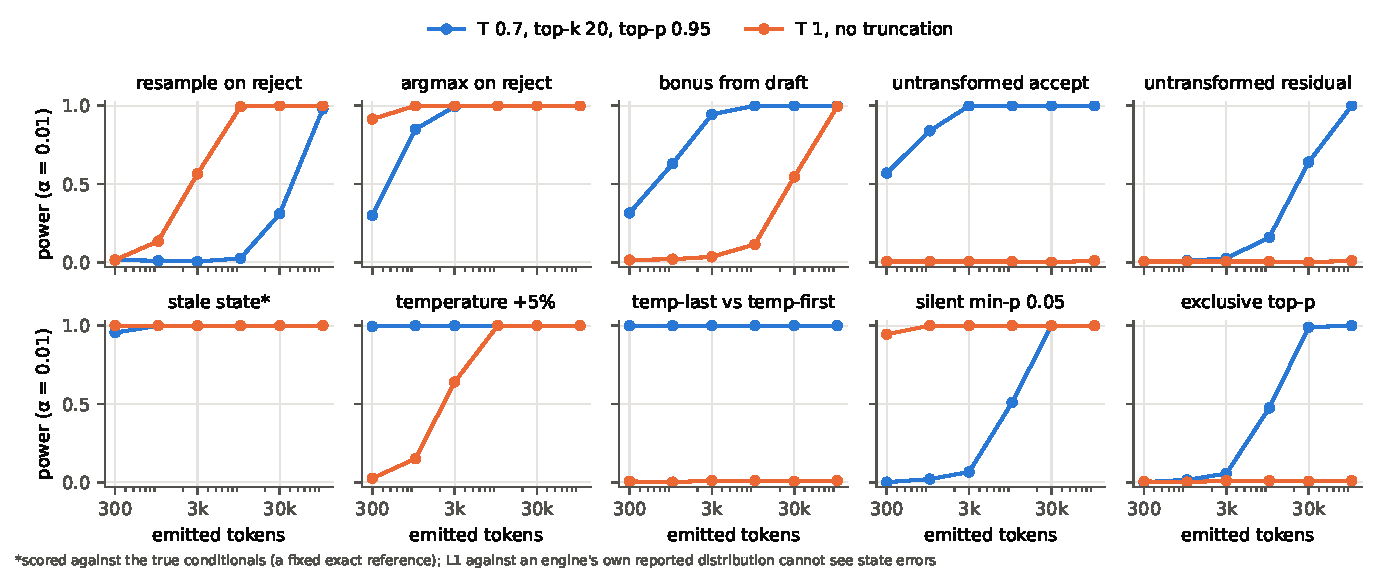
\includegraphics[width=\linewidth]{figures/fig1_power.pdf}
\caption{Power of the pre-specified L1 rule per bug class (any support violation, or the Bonferroni battery; toy LM, seed 0, sequences of about 256 tokens, 200 replications, $\alpha=0.01$). The stale-state curve uses the true conditionals as a fixed reference; L1 against an engine's own reported distribution is blind to it.}\label{fig:power}\end{figure}

\subsection{A natural experiment: the history of an unmerged pull request}\label{sec:natural}
The mlx-lm pull request that adds native MTP (\#990, 37 commits, unmerged) went through several correctness fixes. We use Qwen3.5-4B (bf16, one MTP layer) on 48 fixed prompts, up to 256 tokens each. The prompts were written for this study: short requests mixing code, arithmetic, explanations and creative writing, three of them in Chinese. They are released with the code. ``Thinking'' denotes Qwen's recommended thinking-mode parameters: $T$ 0.6, top-$p$ 0.95, top-$k$ 20.

The runs come from two rounds:
\begin{itemize}
\item \emph{Thinking setting:} all arms come from our second run. Every arm has its own seed, and L1 uses the white-box capture.
\item \emph{$T{=}1$:} the four speculation-on arms come from our first run, which used seed 7 throughout. There L1 is exact without capture, because no truncation is active. L2 and L3 use a new independent-seed speculation-off control.
\end{itemize}
To make the target's verification log-probabilities observable, we apply a one-line reporting patch to the earlier commits. It changes what is yielded, not what is sampled.

\begin{itemize}
\item \textbf{A} (1ff33d5): exact-match verification. The recurrent (GatedDeltaNet) state is not rolled back after a rejected draft. The commit message lists this as a ``known limitation.'' The code comment calls the one-token contamination ``empirically negligible compared to the sequence length'' and adds that ``output may differ slightly.'' The author removed it in the next commit, 24 minutes later.
\item \textbf{B} (673b304): probabilistic acceptance on untransformed log-probabilities; rejection resamples from the target.
\item \textbf{C} (96093cf): acceptance and the residual both use untransformed log-probabilities.
\item \textbf{D} (c4963b1): the head of the pull request.
\end{itemize}
B and C share an additional greedy-mode bug: greedy decoding was detected as \texttt{sampler is None}, but the CLI and server always pass a sampler.

\begin{table}[h]\centering\small
\begin{tabular}{lcccccc}
\toprule
Commit & L1 $T{=}1$ & L1 thinking & L3 $T{=}1$ & L3 thinking & L2 TV ($\times$ floor) & Greedy hazard\\
\midrule
A state & pass & pass & $\le$0.0005 & $\le$0.0005 & 0.33 / 0.16 (53$\times$ / 28$\times$) & 5.5\% \\
B & pass & \textbf{reject} & 0.91 & 0.0015 & floor & 2.7\% \\
C & pass & \textbf{reject} & 0.08 & 0.0010 & floor & 4.4\% \\
D fixed & pass & pass & 0.67 & 0.19 & floor & 0.6\% \\
\bottomrule
\end{tabular}
\caption{Each buggy commit fails at least one test, and the fixed head passes all of them.
L1 decisions follow the pre-specified rule. B is rejected by 15 impossible tokens and surprisal $z=+5.4$; C by 40 impossible tokens, $z=+11.5$ and KS (derandomized $p=0.007$).
L3 entries are Westfall--Young family $p$-values against the independent-seed control, with the bf16 reference.
L2 is the mean per-token TV against a clean prefill at $T{=}1$ / thinking. The speculation-off floor is 0.0063 / 0.0055, from the independent-seed controls.
The greedy hazard is the per-token rate of first divergence from plain greedy decoding (geometric MLE; Kaplan--Meier medians 12, 23, 13 and 123 tokens).}\label{tab:natural}\end{table}

\paragraph{Readings.}
\begin{enumerate}
\item \textbf{The layers separate as predicted.}
  \begin{itemize}
  \item L1 catches B and C at the thinking setting and passes them at $T{=}1$. There only B's resample bug acts, and its effect is below L1's power at 11k tokens.
  \item A passes L1 because it uses exact-match verification: each emitted token is a correct draw from a contaminated distribution. L2 and L3 catch it.
  \item The impossible tokens show the mechanism. B's 15 are all accepted drafts: untransformed acceptance admits drafts outside the declared top-$k$/top-$p$ support. C's 40 are 11 accepted drafts and 29 corrected tokens, because its residual is untransformed too.
  \end{itemize}
\item \textbf{The documented limitation was large.} From the first rejection on, A's per-token TV against a clean prefill is 0.23--0.38 at $T{=}1$ and 0.10--0.22 at the thinking setting; at $T{=}1$ its outputs are 35\% shorter. Position-matched, its excess over the floor is $+0.33$ and $+0.15$ per token (sign-flip $p\le10^{-5}$).
\item \textbf{Greedy identity needs a baseline.} The correct head D diverges from plain greedy decoding at 0.60\% per token (95\% CI 0.43--0.83\%), so 79\% of its 256-token outputs diverge. A, B and C diverge at 4.4--9.1$\times$ that rate ($p<10^{-10}$).

  To see why D diverges, we take teacher-forced prefill logits on the plain sequences. All 38 of D's first divergences sit at a top-2 logit gap at or below the 5th percentile of gaps at other positions; the median gap is 0.125, one bf16 step at that magnitude. The buggy commits' divergences are less concentrated at near-ties: 27--47\% are at or below that percentile.
\item \textbf{Robustness.}
  \begin{itemize}
  \item The derandomized $p$-values agree with these conclusions, except that B's KS evidence depends on the coin (derandomized $p=0.34$). B is rejected by its impossible tokens and its surprisal; under the entropy screen its KS $p$ is 0.004.
  \item Padded fixed-budget versions at $T{=}1$ agree: KS $p=0.08$--$0.72$ across the five arms, none rejecting.
  \item Replaying the engine's bf16 arithmetic moves surprisal by about 0.1.
  \end{itemize}
\end{enumerate}

\paragraph{Pre-registered commits.} To reduce reliance on hand-picked commits, we drew four more by a fixed random rule, before any run: one from the exact-match range after the state fix, two from the range with untransformed acceptance, and one after the acceptance fix. We recorded our predictions for each beforehand. All four L1 predictions held:
\begin{itemize}
\item 2555209 (exact-match) and dcbb45a (after the fix) pass with no violations: KS $p=0.47$ and $0.87$, surprisal $z=-1.30$ and $+1.36$.
\item d737eed and e8a8504 are rejected, with 55 and 17 impossible tokens (surprisal $z=+11.4$ and $+6.4$).
\end{itemize}
The mechanisms match the code. d737eed's residual is untransformed: as for C, its impossible tokens are 16 accepted drafts and 39 corrected tokens. e8a8504 resamples from the target after untransformed acceptance: as for B, all 17 are accepted drafts.

With the bf16 reference, L3 detects d737eed ($p=0.001$) and e8a8504 ($p=0.0045$) and passes the correct commits ($p=0.41$ and $0.032$); with the 4-bit reference only d737eed is detected. Our L3 predictions did not name a reference model, so neither result was pre-specified. On both correct commits, our earlier float32 re-implementation of the sampler would have reported one false ``impossible'' token each.

\begin{figure}[t]\centering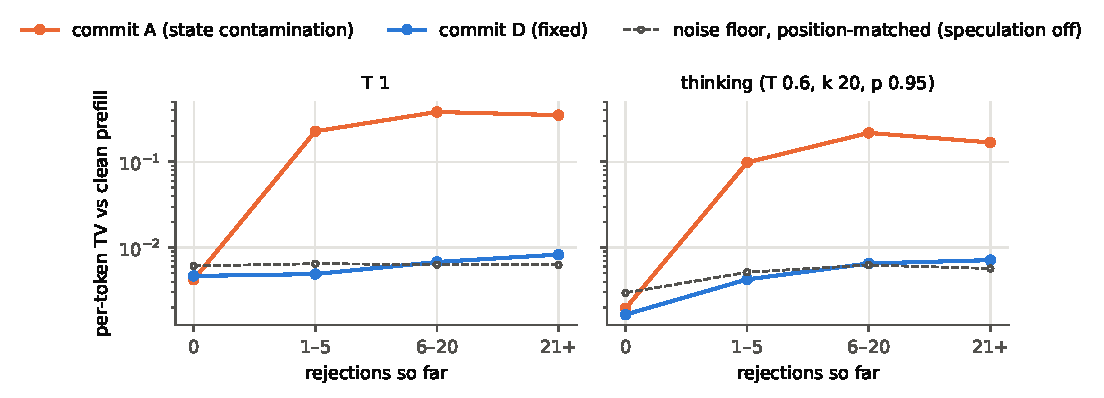
\includegraphics[width=0.9\linewidth]{figures/fig2_dose_response.pdf}
\caption{Per-token TV against a clean prefill, by number of rejections so far, counting the current token's own rejection; the bins are descriptive, not test strata (thinking: independent-seed runs; $T{=}1$: first-run speculation-on arms against the new control). The floor is position-matched for every bin. Over all positions, D does not differ from speculation off (sign-flip $p=0.14$ at $T{=}1$, $0.49$ thinking). In the 21+ bin, B, C and D sit 23--32\% above the matched floor. This could be text selection, since many rejections occur in harder text, or numerical drift after repeated rollbacks; we did not separate the two.}\label{fig:dose}\end{figure}

\section{Audit of local engines}\label{sec:audit}
\begin{table}[h]\centering\small
\begin{tabular}{lllll}
\toprule
Engine & Version & Weights & Speculation & Verification \\
\midrule
kapitsa & 0.2.36 & own 4-bit build & MTP head; DFlash drafter & keyed inverse-CDF \\
MTPLX & 2.12.3 & 4-bit, group 64 (MTPLX build) & MTP & rejection sampling \\
raceline$^*$ & 0.8.0, 0.8.1 & own rotated 4-bit format & MTP & keyed Gumbel, batch-invariant \\
llama.cpp & 0.9.0 (b12110) & Q8\_0 GGUF & draft-MTP, 3 drafts & exact match \\
\bottomrule
\end{tabular}
\caption{Engines audited, all with Qwen3.5-4B on one Apple M6 machine with 24 GB of unified memory. $^*$Developed by the author. Only raceline's sampler could be called directly (white-box); the others were tested through their APIs.}\label{tab:engines}\end{table}

\paragraph{Design.} For each engine we use 32 prompts, 2 samples each, and up to 256 tokens, at $T{=}1$ and at the thinking setting. There are three arms:
\begin{itemize}
\item speculation on;
\item speculation off with the same seeds, for identity;
\item speculation off with independent seeds, for L3.
\end{itemize}
Comparing the two speculation-off arms gives an A/A cell for every engine and setting. Only llama.cpp exposes per-token distributions through its API.

\paragraph{Identity.} Same-seed outputs with speculation on vs.\ off:
\begin{itemize}
\item raceline: 128/128 identical per version, so the per-output divergence rate is at most 2.3\% (95\%);
\item kapitsa: 52--56/64, consistent with the rounding-level differences its documentation describes;
\item MTPLX: 0/64. Its draws are not coupled across modes, and its claim is distributional;
\item llama.cpp: 64/64 at the thinking setting and 53/64 at $T{=}1$.
\end{itemize}

\paragraph{Distribution (L3).} We permute within (prompt, sample) strata and use the 4-bit reference. A cell fails at Westfall--Young $p\le0.01$.
\begin{itemize}
\item No cell fails. Speculation on vs.\ off gives $p=0.12$--$0.91$ at the thinking setting and $0.15$--$0.79$ at $T{=}1$, except llama.cpp at $T{=}1$ ($p=0.033$).
\item One $p\approx0.03$ among about fourteen distinct cells is unremarkable. Its A/A cell gives 0.034, because llama.cpp's speculation-on arm is largely identical to the same-seed off arm.
\item For raceline (both settings) and llama.cpp at the thinking setting, speculation is bit-identical, so the on-vs-off test \emph{is} the A/A test.
\item Across the eight A/A cells the $p$-values range from 0.03 to 0.91.
\end{itemize}
\emph{Positive control under audit conditions.} Commits A and C, rescored with the same 4-bit reference against the independent-seed control, are detected at the thinking setting ($p\le0.001$); B is not ($p=0.42$). At $T{=}1$ only A is detected; C gives $p=0.78$.

From one run per commit, we conclude that the audit would likely detect state errors of A's size, and sampling errors of C's size at the thinking setting. It does not rule out subtle acceptance errors of B's size, which only L1 would see; three of the four APIs expose nothing L1 can use.

\paragraph{Samplers against their declared distribution.} Both deviations were found by reading source code, then confirmed with tests targeted at the hypothesis.
\begin{itemize}
\item \textbf{raceline 0.8.0} keeps only the top 1024 logits when top-$k{=}0$ (``the tail carries no mass''). At $T{=}1$ the mass beyond rank 1024 has mean $7\cdot10^{-4}$ and maximum 7.9\%.

We call 0.8.0's \texttt{\_sample} and C top-$k$ on 2,947 real logit vectors. The mass beyond the stored top-4096 is restored as filler tokens, so the input matches the head and the total tail mass. With 20 seeds each, it emits 0 tokens beyond rank 1024 against 41.5 expected ($p\approx10^{-18}$); the omnibus battery does not detect this (KS $p=0.29$).

We proposed an exact fix that keeps the coupling: draw the tail's maximum as $\mathrm{Gumbel}(\mathrm{logsumexp}_{\text{tail}}/T)$, which is exact by max-stability, and sample within the tail if it wins. Release 0.8.1 implements it. On the identical input, 0.8.1 emits 39 tokens against 41.5 expected, and speculation on and off remain bit-identical.
\item \textbf{kapitsa} sets $K=\mathrm{clamp}(\text{top\_k}\le0\,?\,32:\text{top\_k},1,32)$ in its Qwen3.5 path (\texttt{src/model/qwen35\_spec.cpp}, commit 854ece3). This applies whenever top-$k$ is 0 or above 32, and it is not documented. At $T{=}1$, measured with mlx-lm 4-bit logits, the mass this removes has mean 1.1\% (p99 20.7\%) on non-thinking text and 0.48\% on thinking text.

A black-box rank test agrees. kapitsa emits about 5$\times$ fewer tokens than the other engines beyond reference rank 32, and about 20$\times$ fewer beyond rank 64 (Figure~\ref{fig:rank}). In a minimal reproduction with 400 seeds at $T{=}1$ and top-$k{=}0$, kapitsa yields exactly 32 distinct first tokens. The reference distribution predicts about 121 (99\% interval 103--140 over 20,000 simulations, and never 32 or fewer), and a top-32 cap 31.4. The engines' own weights shift these values somewhat.

We reported this upstream (kapitsa\#1286) and invite the maintainers' response.
\item \textbf{llama.cpp.} We take its pre-sampling top-20 log-probabilities and its declared order: top-$k$ (keeping exactly $k$), top-$p$, min-$p$, then temperature. Plain decoding passes L1 at both settings, with no violations:
  \begin{itemize}
  \item $T{=}1$: 14,354 tokens tested, none screened; KS $p=0.59$, surprisal $z=+0.25$.
  \item Thinking: 16,376 of 16,384 tokens tested, 8 screened at ambiguous top-$p$ boundaries; KS $p=0.65$, $z=-0.16$.
  \end{itemize}
  Post-sampling probabilities would test only the final draw; a silent cap would pass that check. Under draft-MTP, 99.4\% of the reported per-token probabilities are a placeholder $p{=}1$, an open upstream issue (\#27972) that blocks L1 in speculative mode.
\end{itemize}

\begin{figure}[t]\centering
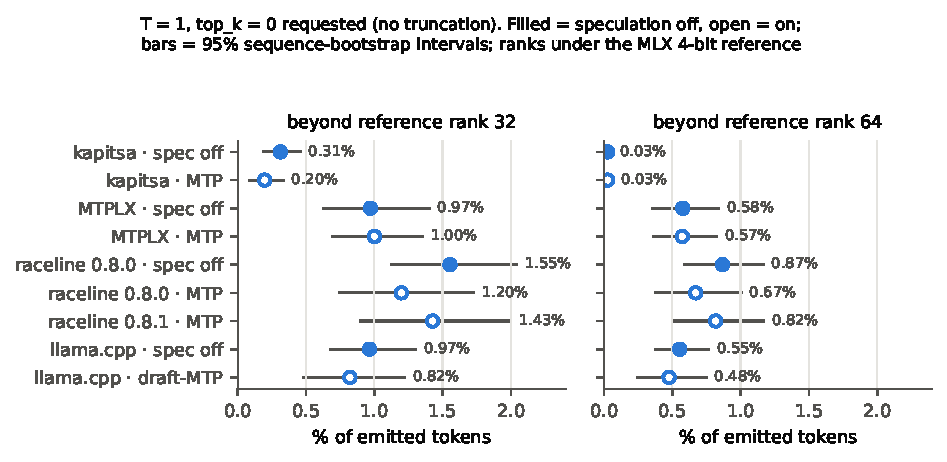
\includegraphics[width=0.62\linewidth]{figures/fig3_rank_support.pdf}\hfill
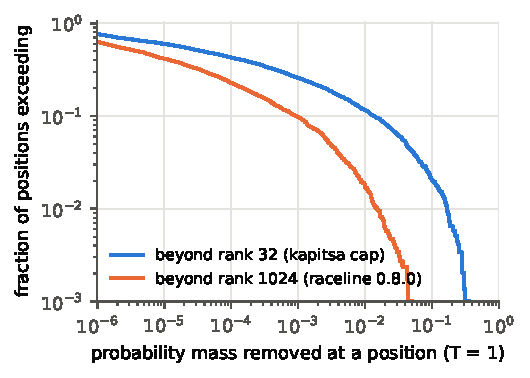
\includegraphics[width=0.36\linewidth]{figures/fig4_tail_mass.pdf}
\caption{Left: share of emitted tokens beyond reference ranks 32 and 64 at $T{=}1$ with top-$k{=}0$ requested (95\% sequence-bootstrap intervals). The engines use different quantizations from the reference, so small counts beyond a rank partly reflect rank disagreement. Right: complementary CDF of the mass that a top-$K$ cutoff removes.}\label{fig:rank}\label{fig:tail}\end{figure}

\paragraph{Sampler semantics.} From each engine's source, the order of operations is:
\begin{itemize}
\item temperature first: HF, vLLM, raceline, MTPLX;
\item temperature last: llama.cpp, mlx-lm, kapitsa.
\end{itemize}
Defaults also differ: llama.cpp's server documents top-$k$ 40, top-$p$ 0.95 and min-$p$ 0.05 unless a request overrides them \cite{llamacppserver}.

For the same logits and Qwen's recommended non-thinking parameters ($T$ 0.7, top-$p$ 0.8, top-$k$ 20; Qwen3.5 model card), mlx-lm's semantics differ from HF's by a mean per-token TV of 0.024, and 2.2\% of the tokens mlx-lm emits are impossible under HF semantics. At the thinking parameters the figures are 0.0078 and 0.9\%.

Transform conformance also measures the arithmetic of the pull request's sampler: mlx-lm's earlier top-$p$, applied to bf16 log-probabilities. Two effects show up against the exact float64 semantics:
\begin{itemize}
\item its truncation set differs at about 3\% of positions (mean per-token TV $4.5\cdot10^{-5}$), because the ascending cumulative sum is accumulated in bf16;
\item including the bf16 temperature scaling, its distribution differs from the declared one by a mean per-token TV of $3.2\cdot10^{-4}$ (p99 $2.9\cdot10^{-3}$, maximum 0.012).
\end{itemize}
The first figure comes from all thinking-setting runs. The second comes from the four pre-registered runs, whose capture replays the bf16 scaling; TV exceeds $10^{-6}$ at 39--40\% of positions. Both effects belong to the sampler function itself, so they are the same with speculation on and off by construction, not by measurement.

\section{Recommendations}
\begin{enumerate}
\item Test at the settings you ship \emph{and} at $T{=}1$ without truncation. Each setting is blind to some bug classes (Table~\ref{tab:taxonomy}). Add tail counts at fixed ranks to catch truncation caps.
\item Separate algorithm from numerics. Report the per-token TV between verification-pass and decode distributions as a noise floor, judge exactness distributionally, and calibrate greedy-identity checks with a per-token hazard baseline.
\item Expose per-token distributions before the sampler transform, with token ids. Even top-20 log-probabilities make an exact L1 possible at truncated settings, provided the engine keeps exactly $k$ tied tokens or the report extends beyond rank $k$. Post-transform probabilities test only the final draw.
\item Document sampler semantics: the order of operations, tie handling, defaults and any implicit truncation. ``top\_k = 0'' should mean no truncation.
\item Combine first-token counting at fixed prefixes, which sees verification and rejection-path errors directly at the first position, with L1 on natural sequences, which also sees bonus and history-dependent errors.
\item Couple randomness deliberately when bit-identity matters. With batch-invariant kernels, keyed noise \cite{daliri2024} makes speculation bit-identical and identity checks meaningful. Independent samples then need distinct seeds.
\end{enumerate}

\section{Related work}
\begin{itemize}
\item \textbf{Sequential PIT.} The randomized PIT comes from forecast evaluation \cite{dgt1998,czado2009}, and its sequential validity from the prequential framework \cite{dawid1984,smdawid1993,rosenblatt1952,brockwell2007}. Randomized quantile residuals are the same idea for GLMs \cite{dunnsmyth1996}. Randomized and fuzzy $p$-values \cite{geyermeeden2005,habigerpena2011} and averaging-based merging \cite{vovkwang2020} inform our derandomization.
\item \textbf{Testing samplers.} The closest work tests samplers statistically:
  \begin{itemize}
  \item posterior-quantile and joint-distribution tests of Bayesian software \cite{cook2006,geweke2004,talts2018};
  \item unit tests for MCMC code \cite{grosse2014,gandyscott2020};
  \item testing of constrained samplers \cite{chakraborty2019,meel2020};
  \item fuzzing of probabilistic programming systems \cite{probfuzz2018}.
  \end{itemize}
\item \textbf{Speculative decoding.} Speculative sampling \cite{leviathan2023,chen2023} has drafters such as Medusa and EAGLE \cite{medusa2024,eagle2024} and multi-draft verification \cite{spectr2023}. Drafter-invariant coupling \cite{daliri2024} and Gumbel constructions \cite{maddison2014,kool2019} underlie keyed-noise verification and our tail construction.
\item \textbf{Auditing and verification.} Model-equality testing \cite{gao2024}, rank-based uniformity tests \cite{rut2025} and audits of model substitution \cite{cai2025} check which model an API serves. TOPLOC \cite{toploc2025} verifies inference by hashing activations. Our tests instead check the sampling algorithm against its declared distribution.
\item \textbf{Engine-level checks.}
  \begin{itemize}
  \item vLLM's unit tests apply $\chi^2$ goodness-of-fit to its rejection sampler on synthetic target and draft distributions. Its end-to-end test compares the distribution of whole answers to one fixed prompt, with and without speculation \cite{vllmtests}; a whole-output comparison can in principle see later-position errors.
  \item ``Lossless but Not Free'' \cite{lossless2026} uses a $\chi^2$ test.
  \item An upstream llama.cpp report counted the token that follows a given first generated token after a fixed prompt, on a tiny random model \cite{llamacpp29975}.
  \end{itemize}
  Section~\ref{sec:toy} compares first-token counting with L1.
\item \textbf{Nondeterminism.} Lossy verification \cite{lossy2026}, reproducibility across backends \cite{silent2026,yuan2025}, batch-invariant kernels \cite{tm2025}, and anytime-valid inference \cite{ramdas2023}, which would allow continuous monitoring. Westfall--Young resampling \cite{westfallyoung1993} gives our family $p$-values.
\end{itemize}

\section{Limitations}
\begin{itemize}
\item \textbf{Scope.} One hybrid-SSM model family; MTP with one draft per step (three for llama.cpp); outputs up to 256 tokens; batch size 1; Apple silicon only, with no CUDA engines.
\item \textbf{The natural experiment is retrospective.} Its commits were labeled by the author's own fixes, and four additional commits were drawn by a fixed rule.
\item \textbf{One run per positive control and per cell.}
\item \textbf{The toy is small.} It shows mechanisms, not real-world power.
\item \textbf{White-box arithmetic.} The bf16 replay assumes the compiled kernel rounds like eager execution.
\item \textbf{L1 coverage in the audit.} Three of four APIs expose no per-token distributions, and llama.cpp's become placeholders under speculation. L1 coverage of speculative modes in the audit therefore rests on source reading, targeted tests and L3, which does not rule out subtle acceptance errors.
\item \textbf{Small deviations.} Per-token deviations of TV $\delta$ need roughly $N\gg\delta^{-2}$ tokens: about $10^6$ for $\delta=10^{-3}$.
\end{itemize}

\paragraph{Disclosure and fairness.}
\begin{itemize}
\item raceline is developed by the author of this paper. Its deviation was found by the same source reading as kapitsa's, and it was tested with the same scripts. Its sampler could also be called directly, which the other engines did not allow. Its fix uses our construction.
\item The pull-request commits were never merged and were fixed by their author. We cite their hashes and keep a git bundle of all 37 commits (SHA-256 \texttt{86d632cb\ldots{}a8c}), so the code stays available if the history is rewritten.
\item \emph{AI assistance.} This work was carried out with substantial assistance from an AI system (Anthropic's Claude), which wrote most of the code and text under the author's direction. The AI system is not an author; the author takes full responsibility for the content.
\item All numbers are produced by the released scripts.
\end{itemize}

\begin{thebibliography}{99}\small
\bibitem{leviathan2023} Y. Leviathan, M. Kalman, Y. Matias. Fast inference from transformers via speculative decoding. ICML 2023.
\bibitem{chen2023} C. Chen et al. Accelerating large language model decoding with speculative sampling. arXiv:2302.01318, 2023.
\bibitem{rosenblatt1952} M. Rosenblatt. Remarks on a multivariate transformation. Annals of Mathematical Statistics 23(3), 1952.
\bibitem{dawid1984} A. P. Dawid. Statistical theory: the prequential approach. JRSS A 147(2), 1984.
\bibitem{smdawid1993} F. Seillier-Moiseiwitsch, A. P. Dawid. On testing the validity of sequential probability forecasts. JASA 88(421):355--359, 1993.
\bibitem{brockwell2007} A. Brockwell. Universal residuals: a multivariate transformation. Statistics \& Probability Letters 77(14):1473--1478, 2007.
\bibitem{dunnsmyth1996} P. Dunn, G. Smyth. Randomized quantile residuals. JCGS 5(3):236--244, 1996.
\bibitem{czado2009} C. Czado, T. Gneiting, L. Held. Predictive model assessment for count data. Biometrics 65(4), 2009.
\bibitem{dgt1998} F. Diebold, T. Gunther, A. Tay. Evaluating density forecasts. International Economic Review 39(4), 1998.
\bibitem{geyermeeden2005} C. Geyer, G. Meeden. Fuzzy and randomized confidence intervals and p-values. Statistical Science 20(4):358--366, 2005.
\bibitem{habigerpena2011} J. Habiger, E. Pe\~na. Randomised P-values and nonparametric procedures in multiple testing. Journal of Nonparametric Statistics 23(3):583--604, 2011.
\bibitem{vovkwang2020} V. Vovk, R. Wang. Combining p-values via averaging. Biometrika 107(4):791--808, 2020.
\bibitem{doob1936} J. L. Doob. Note on probability. Annals of Mathematics 37(2):363--367, 1936.
\bibitem{halmos1939} P. R. Halmos. Invariants of certain stochastic transformations: the mathematical theory of gambling systems. Duke Mathematical Journal 5(2):461--478, 1939.
\bibitem{westfallyoung1993} P. Westfall, S. Young. Resampling-Based Multiple Testing. Wiley, 1993.
\bibitem{cook2006} S. Cook, A. Gelman, D. Rubin. Validation of software for Bayesian models using posterior quantiles. JCGS 15(3):675--692, 2006.
\bibitem{geweke2004} J. Geweke. Getting it right: joint distribution tests of posterior simulators. JASA 99(467):799--804, 2004.
\bibitem{talts2018} S. Talts et al. Validating Bayesian inference algorithms with simulation-based calibration. arXiv:1804.06788, 2018.
\bibitem{grosse2014} R. Grosse, D. Duvenaud. Testing MCMC code. NIPS Workshop on Software Engineering for Machine Learning, 2014. arXiv:1412.5218.
\bibitem{gandyscott2020} A. Gandy, J. Scott. Unit testing for MCMC and other Monte Carlo methods. arXiv:2001.06465, 2020.
\bibitem{chakraborty2019} S. Chakraborty, K. S. Meel. On testing of uniform samplers. AAAI 2019.
\bibitem{meel2020} K. S. Meel, Y. Pote, S. Chakraborty. On testing of samplers. NeurIPS 2020 (arXiv:2010.12918).
\bibitem{probfuzz2018} S. Dutta, O. Legunsen, Z. Huang, S. Misailovic. Testing probabilistic programming systems. ESEC/FSE 2018.
\bibitem{medusa2024} T. Cai et al. Medusa: simple LLM inference acceleration framework with multiple decoding heads. ICML 2024 (arXiv:2401.10774).
\bibitem{eagle2024} Y. Li et al. EAGLE: speculative sampling requires rethinking feature uncertainty. ICML 2024 (arXiv:2401.15077).
\bibitem{spectr2023} Z. Sun, A. T. Suresh, J. H. Ro, A. Beirami, H. Jain, F. Yu. SpecTr: fast speculative decoding via optimal transport. NeurIPS 2023 (arXiv:2310.15141).
\bibitem{daliri2024} M. Daliri, C. Musco, A. T. Suresh. Coupling without communication and drafter-invariant speculative decoding. arXiv:2408.07978, 2024.
\bibitem{maddison2014} C. J. Maddison, D. Tarlow, T. Minka. A* sampling. NIPS 2014 (arXiv:1411.0030).
\bibitem{kool2019} W. Kool, H. van Hoof, M. Welling. Stochastic beams and where to find them: the Gumbel-top-k trick for sampling sequences without replacement. ICML 2019.
\bibitem{gao2024} I. Gao, P. Liang, C. Guestrin. Model equality testing: which model is this API serving? arXiv:2410.20247, 2024.
\bibitem{rut2025} Auditing black-box LLM APIs with a rank-based uniformity test. arXiv:2506.06975, 2025.
\bibitem{cai2025} W. Cai, T. Shi, X. Zhao, D. Song. Are you getting what you pay for? Auditing model substitution in LLM APIs. arXiv:2504.04715, 2025.
\bibitem{toploc2025} J. M. Ong et al. TOPLOC: a locality sensitive hashing scheme for trustless verifiable inference. ICML 2025 (arXiv:2501.16007).
\bibitem{lossless2026} Lossless but not free: an empirical anatomy of speculative decoding on consumer hardware. arXiv:2607.17283, 2026.
\bibitem{lossy2026} Revisiting lossy verification in speculative decoding. arXiv:2607.26627, 2026.
\bibitem{silent2026} D. Pape, J. Evertz, L. Sch\"onherr. The silent hyperparameter: quantifying the impact of inference backends on LLM reproducibility. arXiv:2605.19537, 2026.
\bibitem{yuan2025} J. Yuan et al. Give me FP32 or give me death? Challenges and solutions for reproducible reasoning. arXiv:2506.09501, 2025.
\bibitem{tm2025} Thinking Machines Lab. Defeating nondeterminism in LLM inference. 2025.
\bibitem{ramdas2023} A. Ramdas, P. Gr\"unwald, V. Vovk, G. Shafer. Game-theoretic statistics and safe anytime-valid inference. Statistical Science 38(4):576--601, 2023.
\bibitem{mtplxreadme} MTPLX 2.12.3, package README (PyPI distribution metadata), accessed November 2026.
\bibitem{racelinereadme} raceline README, releases 0.8.0 and 0.8.1, accessed November 2026.
\bibitem{llamacppserver} llama.cpp, \texttt{tools/server/README.md} (sampling defaults), release b12110, accessed November 2026.
\bibitem{vllmtests} vLLM project. tests/v1/spec\_decode/test\_rejection\_sampler\_utils.py and tests/v1/e2e/spec\_decode/test\_distribution\_shift.py. GitHub, accessed November 2026.
\bibitem{llamacpp23302} llama.cpp issue \#23302: draft-mtp changes deterministic output with --spec-draft-n-max 3 on Qwen3.6 MTP model. GitHub, May 2026.
\bibitem{llamacpp25618} llama.cpp issue \#25618: speculative decoding (draft-mtp / draft-dspark): greedy output diverges from vanilla on quantized targets. GitHub, July 2026.
\bibitem{llamacpp29975} llama.cpp issue \#29975: llama-speculative changes the distribution at temp $>$ 0. GitHub, October 2026.
\end{thebibliography}
\end{document}
